\section{Server side}
\NomeProgetto{} è una web application che non richiede un'ampia comunicazione con il lato server. Esso è infatti utilizzato solo per l'interrogazione del database PostgreSQL per permettere all'utente di caricare i suoi dati contenuti nel database. \\
Per questo motivo è stato deciso di non adottare una specifica architettura lato server. \\
I file dedicati sono contenuti nella cartella \texttt{server} e così organizzati:
\begin{itemize}
	\item \texttt{test} è la sottocartella contenente il file \textbf{server.test.js} utile a controllare che la connessione con il server avvenga correttamente; 
	\item \texttt{config} è la sottocartella contenente i file per la configurazione del database. All'interno del file \textbf{default.js} è infatti possibile cambiare i dati di acceso al DB con le proprie credenziali (figura \ref{config}).
	Nel file \textbf{db.js} avviene l'effettiva connessione con il database;
	\item \texttt{api} è la sottocartella contenente il file \textbf{DataSet.js}. Al suo interno sono presenti le API create con Express.js per la comunicazione del lato client dell'applicazione con il server sviluppato con Node.js.
\end{itemize}

\begin{figure}[hb]
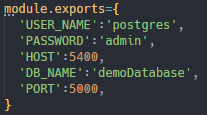
\includegraphics[width=8cm]{Images/credenziali}
\centering
\caption{Credenziali di default}
\label{config}
\end{figure}